\documentclass[12pt,a4paper,oneside]{article}

\usepackage[utf8]{inputenc}
\usepackage[portuguese]{babel}
\usepackage[T1]{fontenc}
\usepackage{amsmath}
\usepackage{amsfonts}
\usepackage{amssymb}
\usepackage{graphicx}
\usepackage{hyperref}

\usepackage{listings}
\usepackage{xcolor}

\definecolor{mygreen}{rgb}{0,0.6,0}
\definecolor{mygray}{rgb}{0.5,0.5,0.5}
\definecolor{mymauve}{rgb}{0.58,0,0.82}

\lstdefinelanguage{JavaScript}{
  keywords={typeof, new, true, false, catch, function, return, null, catch, switch, var, if, in, while, do, else, case, break},
  keywordstyle=\color{blue}\bfseries,
  ndkeywords={class, export, boolean, throw, implements, import, this},
  ndkeywordstyle=\color{darkgray}\bfseries,
  identifierstyle=\color{black},
  sensitive=false,
  comment=[l]{//},
  morecomment=[s]{/*}{*/},
  commentstyle=\color{purple}\ttfamily,
  stringstyle=\color{red}\ttfamily,
  morestring=[b]',
  morestring=[b]",
}

\lstset{ %
  backgroundcolor=\color{white},   % choose the background color; you must add \usepackage{color} or \usepackage{xcolor}
  basicstyle=\small,        % the size of the fonts that are used for the code
  breakatwhitespace=false,         % sets if automatic breaks should only happen at whitespace
  breaklines=true,                 % sets automatic line breaking
  captionpos=b,                    % sets the caption-position to bottom
  commentstyle=\color{mygreen},    % comment style
  deletekeywords={...},            % if you want to delete keywords from the given language
  escapeinside={\%*}{*)},          % if you want to add LaTeX within your code
  extendedchars=true,              % lets you use non-ASCII characters; for 8-bits encodings only, does not work with UTF-8
  frame=single,	                   % adds a frame around the code
  keepspaces=true,                 % keeps spaces in text, useful for keeping indentation of code (possibly needs columns=flexible)
  keywordstyle=\color{blue},       % keyword style
  language=HTML,                 % the language of the code
  otherkeywords={*,...},           % if you want to add more keywords to the set
  numbers=left,                    % where to put the line-numbers; possible values are (none, left, right)
  numbersep=5pt,                   % how far the line-numbers are from the code
  numberstyle=\tiny\color{mygray}, % the style that is used for the line-numbers
  rulecolor=\color{black},         % if not set, the frame-color may be changed on line-breaks within not-black text (e.g. comments (green here))
  showspaces=false,                % show spaces everywhere adding particular underscores; it overrides 'showstringspaces'
  showstringspaces=false,          % underline spaces within strings only
  showtabs=false,                  % show tabs within strings adding particular underscores
  stepnumber=1,                    % the step between two line-numbers. If it's 1, each line will be numbered
  stringstyle=\color{mymauve},     % string literal style
  tabsize=2,	                   % sets default tabsize to 2 spaces
  title=\lstname,                   % show the filename of files included with \lstinputlisting; also try caption instead of title
  moredelim=**[is][\color{purple}]{@}{@},
}

\author{\\Universidade Federal de Goiás - UFG (Regional Jataí) \\Bacharelado em Ciência da Computação \\Física para Ciência da Computação \\Prof. Esdras Lins Bispo Jr.}

\title{
	{\sc \huge Lista de Exercícios 4} 
	\\{\tt Versão 1.0}
}

\begin{document}

\maketitle

\begin{enumerate}

\section{Conceitos}
	
	\item {\bf (Halliday PG.4.5)} A Figura 1 mostra três situações nas quais projéteis iguais são lançados do solo (a partir do mesmo nível) com a mesma velocidade escalar e o mesmo ângulo. Entretanto, os projéteis não caem no mesmo terreno. Ordene as situações de acordo com a velocidade escalar final dos projéteis imediatamente antes de aterrissarem, começando pela maior. 
	
	\begin{figure}[htb]
		\begin{center}
			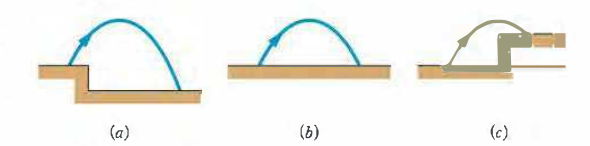
\includegraphics[scale=0.8]{imagens/fig1}
		\end{center}
		\caption{Lançamento de projéteis em três situações diferentes.}
	\end{figure}
	
	\item {\bf (Halliday 4.21)} Um dardo é arremessado horizontalmente com uma velocidade inicial de 10 m/s em direção a um ponto P, o centro de um alvo de parede. O dardo atinge um ponto Q do alvo, verticalmente abaixo de P, 0,19 s depois do arremesso. \label{q:dardo}
		\begin{enumerate}
			\item Qual é a distância PQ?
			\item A que distância do alvo foi arremessado o dardo?
		\end{enumerate}	
	
	\item {\bf (Halliday PG.7.10)} Uma bola é arremessada ou deixada cair a partir do repouso da borda de um precipício. Qual dos gráficos na Figura 2 poderia mostrar como a energia cinética da bola varia durante a queda?	 \label{q:bola}
	
	\begin{figure}[htb]
		\begin{center}
			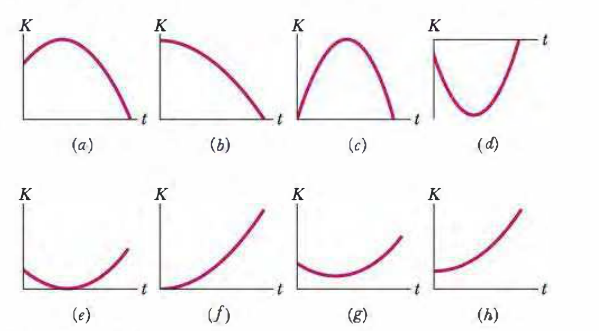
\includegraphics[scale=0.8]{imagens/fig2}
		\end{center}
		\caption{Opções de gráficos para a queda da bola.}
	\end{figure}	


\section{Programação}

	\item[] {\bf Observação:} Para as duas questões a seguir, use como base o código disponível em \url{https://github.com/bispojr/biblioteca-fisica}.

	\item Em JavaScript, reescreva as funções {\tt valoresIniciais} e {\tt emCadaPasso} de forma que exista uma bola representando o movimento do dardo da Questão \ref{q:dardo} desta lista. Admita que a velocidade inicial seja de 50 px/s e $g$ = 9,8 px/s$^2$.
	
	\item Em JavaScript, reescreva as funções {\tt valoresIniciais} e {\tt emCadaPasso} de forma que exista uma bola que represente o movimento da bola da Questão \ref{q:bola} desta lista. Também represente o precipício como um bloco que tenha uma altura de 300 px (tendo como referência a base inferior do canvas). Acrescente o fato de que a bola quicará no solo até o repouso. Admita que em cada colisão com o solo, a bola transfere 20\% de sua energia cinética.
		
\end{enumerate}

\section{Referências}

\begin{itemize}
	\item HALLIDAY, D.; RESNICK, R.. Fundamentos de Física. Volume 1, Mecânica. 8ª Edição, LTC, Rio de Janeiro, 2011.

	\item RAMTAL, D.; DOBRE, A. Physics for JavaScript Games, Animation, and Simulations with HTML5 Canvas, Apress, 2014.
\end{itemize}

\end{document}